We wrote all of the code in Python 3.10.6 with the usage of the scikit-learn library for preprocessing, and evaluation \cite{scikit-learn}. 
For plausibility, a Bayesian network structure definition and parametrization methods of the package pgmpy \cite{pgmpy} was used. For this, all null representations were standardized. Data was prepossessed with the removal of features with high missing rates ($>$ 80\% overall). All missing value representations were standardized. The imputation process was performed with the median for continuous and a new category (NULLIMP) for categorical variables. Then, the continuous variables were discretized into three bins defined by quantile. The evaluation was with a holdout dataset for each column as the target. Z-Scores were defined for all continuous variables based on the inter-quartile range. Then, rows were also assessed with distance analysis, with Local Outlier Factor and Elliptic Envelope from scikit-learn and the outlier-tree algorithm. We also added a rule engine, using the great\_expectations package. Rules were defined by the team, focusing on impossible numbers present in age, weight or relationship between variables. As for missing information was created with all the data, creating the scoring based on the inverse of the missing percentage. Missing detection was based on primary key variables.
For completeness, we used the inverse of the percentage of nulls in the training set.
The API for serving the prediction models was developed with FastAPI. So, the methods applied in terms of the DQA framework are described in the table \ref{tab:methods}.

\begin{table}[htpb]
\caption{Implemented Methods for data quality assessment} 
\renewcommand{\arraystretch}{1.4}
\setlength{\tabcolsep}{10pt}

\begin{tabularx}{\textwidth}{ p{2cm} p{3.5cm} X }
\hline
 Category   & Subcategory           & Method   \\ \hline
Completeness     & N/A               & Score by the inverse percentage of missing in the train data         \\ 
Plausibility & Atemporal Plausibility & Bayesian model prediction based on the other values of row \\ 
Plausibility & Atemporal Plausibility         & Z-score for column value based on IQR train data       \\    
Plausibility & Atemporal Plausibility           & Elliptic Envelope                       \\ 
Plausibility & Atemporal Plausibility           & Local Outlier Factor                \\ 
Conformance & Value Conformance           & Manual Rule engine                           \\ 
Plausibility & Atemporal Plausibility           & Manual Rule engine                      \\ 
Plausibility & Atemporal Plausibility           & outlier-tree                      \\ 
\hline
\end{tabularx}
\label{tab:methods}
\end{table}
The method of scoring was to obtain a single value that could grasp the quality of the row or patient.
%TC:ignore
%\begin{figure}[htbp]
%\centering
%\caption{Scoring Method}\label{fig:scoring} 
%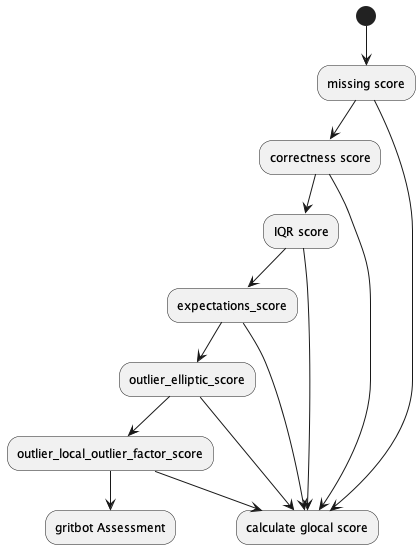
\includegraphics[scale=0.38]{imgs/workflow.png}
%\end{figure}
%TC:endignore

To assess the tool's usefulness, we will implement it in a production environment and collect metrics regarding the data being produced. Then we intended to present some of the results to obstetrics clinicians for them to assess how likely the information is to be suitable for usage.

